\section{Research Problems}
\subsection{Data Representations}\label{sec:data_representation}

Whiles data types mentioned in Sec.~\ref{sec:intro} could be suitable to immersive video streaming,
Their pros and cons are unknown.
In our research group, we have studied 3DoF VR streaming in the past few years \cite{FYHH20,FLPH19}. 
These works help us to understand the existing streaming techniques in 3DoF 360{\degree} video streaming.
We are currently expanding our research to different 6DoF data types to understand their pros and cons.
We will also concretize their suitable usage scenarios.
The final outcome of this work is several immersive video streaming testbeds that support heterogeneous data representations.
Through real experiments, we get to know more systems challenges in these emerging applications.
\subsection{Optimal Streaming}\label{sec:optimal_streaming}

To reduce the bandwidth and computing requirements of immersive video streaming, the streaming systems must be optimized.
In our recent work \cite{mm20_tr},
we adopt Test Model for Immersive Video (TMIV)~\cite{mpeg_N18470,mpeg_N18577,mpeg_N18795}, 
which is a Depth Image Based Rendering (DIBR) codec from MPEG, to optimize the immersive video streaming.
We develop algorithms to solve the configuration optimization problem based on deep learning, particularly the Neural Network (NN) approaches.
The two proposed algorithms are:
a Convolutional Neural Network (CNN) based algorithm and a Deep Reinforcement Learning (DRL) based algorithm
Our CNN algorithm benefits from: (i) automatic extracting latent features and 
(ii) inferencing the prediction rapidly and directly according to the input, which allows the configuration optimizer to 
adapt to various video scenes and dynamic camera parameters.
Our DRL algorithm systematically builds an {\em agent} that can adapt to dynamic {\em environments}~\cite{SB18,PZWL+19,HZZS18,CIZI+19}.
The trained agent learns how to quickly search through a large space for optimal configurations. 
The two proposed algorithms are
trained to adaptively find the optimal configurations given the diverse video content, HMD user behaviors, and user-specified utility functions.
We submitted our paper to ACM Multimedia Conference 2020, which is under review.

We are currently extending this work into a journal submission. 
In particularly, we plan to (i) design, implement, and evaluate an end-to-end DIBR-based immersive video streaming system,
(ii) apply the state-of-the-art DRL algorithms and (iii) adopt larger datasets to train our optimizers.
We expect the performance of our systems can be improved after we apply these optimization techniques.
Moreover, according to the research outcomes of Sec.~\ref{sec:data_representation}, 
% we also study the new streaming technique to address the challenges in these data types.
we will generalize our solutions to other data types/representations.
\subsection{Quality of Experience (QoE)}
To measure QoE of users, we plan to design and conduct a series of user studies  
to quantify the relationship between each parameters and user experience in immersive video streaming sessions.
In our previous work \cite{mm20_tr}, we conduct a small-scale user study to evaluate our solution.
The testbed used in that work can be extended and used in more comprehensive subjective experiments.
The high-level architecture of the immersive video streaming system is shown in Fig.~\ref{fig:architecture}.
We also plan to measure the Just-Noticeable Difference (JND)~\cite{JLK06} bitrate of immersive video streaming.
Using JND bitrates, we can intelligently save the network and computing resources without affecting the user experience.
Combining the outcomes of the QoE study with the ones achieved in Sec.~\ref{sec:data_representation} and Sec.~\ref{sec:optimal_streaming}
gives a fully-optimized immersive 6DoF video streaming system.
\begin{figure}[tbh]
	\begin{center}
		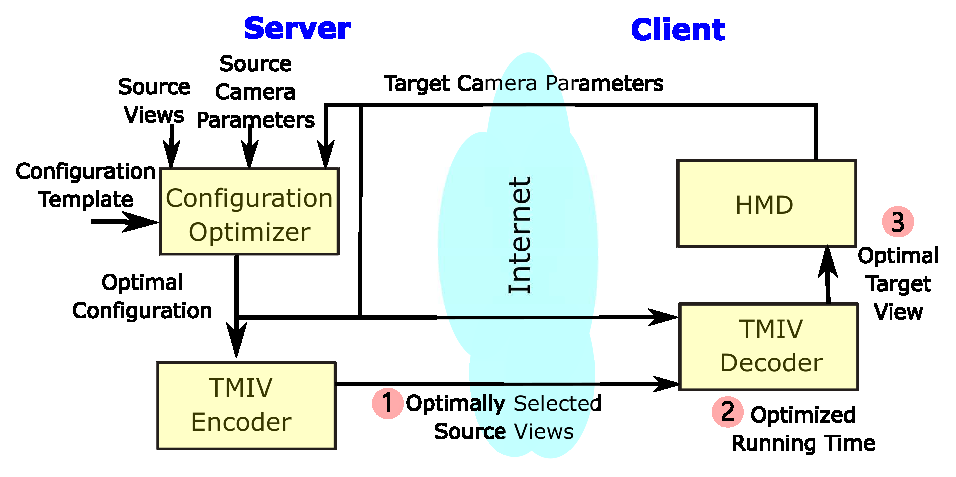
\includegraphics[width=.5\textwidth]{fig/architecture}
		\caption{High-level architecture of immersive video streaming systems for our QoE study.}
		\label{fig:architecture}
	\end{center}
\end{figure}
% If we figure out which level of distortion can tolerate by user, we can choose suitable quality to stream.
% In this way, the bandwidth consumption can be reduced, and the user can perceive the great quality in the same time.
% % However, measuring QoE in immersive video is harder than traditional 2D video or 360{\degree} video.
% The immersive video is the new interactive way in VR,
% so measuring QoE in immersive video is not be researched comprehensively.
% However, it is harder than traditional 2D video or 360{\degree} video.
% In 2D video, the user see the same content on the screen.
% In immersive video and 360{\degree}, user can watch video in different positions and/or orientations by HMD. 
% Each user may see the different content in the video. It makes analyzing the general QoE pattern hard.

% In this research plan, we plan to design a series of experiments to analyze the QoE and user pattern in immersive video.
% We will try different method to overcome the aforementioned problem, 
% including record the trajectory of viewport of subjects, guide subjects where should watch etc..
% Moreover, we plan to measure the Just-Noticeable Difference (JND)~\cite{JLK06} in immersive video.
% In this way, we can find the "sweet point" between QoE and bandwidth consumption.



% \subsection*{First Year: TMIV Immersive Video Streaming System and Explore Data type of 6DoF}
% Given that the current research is the first work trying to optimize the TMIV configurations, we believe
% it will stimulate many more systems research in immersive video streaming. Nevertheless, several crucial
% challenges still need to be overcomed in our first work.
% \begin{itemize}
%     \item {\bf immersive video streaming system:} Currently, because of the high demand for bandwidth
%     and computing resources, build the complete immersive video streaming system is still challenging.
%     In future work, to address the challenges, we add the configuration optimizer into the
%     system. We also design the threshold of bandwidth consumption to limit the maximum of data size.
%     Moreover, we use GPU to process the computation in the system parallelly.
%     \item {\bf State-of-the-art RL algorithm:} In our current work, we choose Deep Q-learning (a.k.a. Deep QNetwork,
%     DQN) to train the DRL configuration optimizer. The experiment shows that DQN achieves
%     better performance. However, there are some methods we haven’t try, e.g., policy gradient, Asynchronous
%     Advantage Actor-critic (A3C). In future work, we seek more powerful DRL algorithms to
%     improve the performance of our DRL optimizer.
%     \item {\bf More experienced optimizer:} In future work, to let our optimizer more general, we train our agent
%     with more datasets. We use more different datasets so that optimizer can choose the best option in
%     most of situation, even the situation they never meet it.
% \end{itemize}

% Moreover, the other data types mention in Sec.~\ref{sec:motivation} also have big potential to be 
% the ideal data representation in immersive video streaming. 
% We plan to study all of 6DoF data types comprehensively to figure out their pros. and cons..
% We also analyze the research problem in each 6DoF data type, respectively.
% % After that, we can know the most important problem in immersive video streaming.

% \subsection*{Second Year: Quality of Experience in Immersive Video Streaming}

% Quality of Experience (QoE) study is important in immersive video streaming. 
% If we figure out which level of distortion can tolerate by user, we can choose suitable quality to stream.
% In this way, the bandwidth consumption can be reduced, and the user can perceive the great quality in the same time.
% % However, measuring QoE in immersive video is harder than traditional 2D video or 360{\degree} video.
% The immersive video is the new interactive way in VR,
% so measuring QoE in immersive video is not be researched comprehensively.
% However, it is harder than traditional 2D video or 360{\degree} video.
% In 2D video, the user see the same content on the screen.
% In immersive video and 360{\degree}, user can watch video in different positions and/or orientations by HMD. 
% Each user may see the different content in the video. It makes analyzing the general QoE pattern hard.

% In this research plan, we plan to design a series of experiments to analyze the QoE and user pattern in immersive video.
% We will try different method to overcome the aforementioned problem, 
% including record the trajectory of viewport of subjects, guide subjects where should watch etc..
% Moreover, we plan to measure the Just-Noticeable Difference (JND)~\cite{JLK06} in immersive video.
% In this way, we can find the "sweet point" between QoE and bandwidth consumption.

% \subsection*{Third Year: Optimize Immersive video streaming}

% Using ABR, synthesis or other method to reduce bandwidth demand and latency.

% \subsection*{Forth Year: Real-Time Immersive Video Streaming System}

% Build the Real-Time Immersive Video Streaming System.




% In second year, we want to propose some new algorithms and techniques to deal with the challenges in 6DoF VR streaming.
% This challenges including but not limited: 
% \begin{itemize}
%     \item {\bf high bandwidth consumption and storage space demand: } The 6DoF data type usually have huge data size, because they have to
%     include all of information in the scene. Take light field video for example, it's expected to require bandwidth in the range between 200 Gb/s 
%     and 1 Tb/s \cite{CVRW+20}, which higher than the highest bandwidth we can achieve today. 
%     \item {\bf low latency demand: } To achieve real-time 6DoF VR video streaming, the low and stable latency is needed. Especially in 
%     interactive application, e.g., holographic conference, gaming. 
% \end{itemize}
% Although there are some existing research work on them \cite{CVRW+20}, it still have lots of problem and challenge need to  be addressed.




